\documentclass[dvipsnames,tikz]{standalone}
\usepackage{amsmath}
\usepackage{xcolor}
\usepackage{tikz}
\usetikzlibrary{calc}
\usetikzlibrary{decorations.pathreplacing,calligraphy,3d}
\usetikzlibrary{positioning}

\tikzset{main/.style={draw=black, circle, color=black}}

\begin{document}
	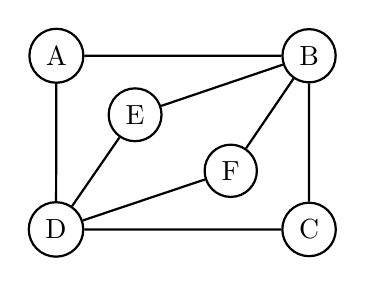
\begin{tikzpicture}[node distance={15mm}, thick] 
		\node[main] (A) {A}; 
		\node[main] (B) [right=2.5cm of A] {B};
		\node[main] (C) [below=1.5cm of B] {C}; 
		\node[main] (D) [left=2.5cm of C] {D};
		\node[main] (E) [below right=0.25cm and 0.5cm of A] {E}; 
		\node[main] (F) [above left=0.25cm and 0.5cm of C] {F}; 
		
		\begin{scope}[font=\tiny]
			\draw[main] (A) -- (B) -- (C) -- (D) -- (A);
			\draw[main] (D) -- (E) -- (B) -- (F) -- (D);
		\end{scope}
	\end{tikzpicture} 
	
	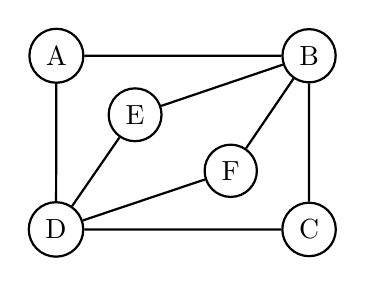
\begin{tikzpicture}[node distance={15mm}, thick] 
		\node[main] (A) {A}; 
		\node[main] (B) [right=2.5cm of A] {B};
		\node[main] (C) [below=1.5cm of B] {C}; 
		\node[main] (D) [left=2.5cm of C] {D};
		\node[main] (E) [below right=0.25cm and 0.5cm of A] {E}; 
		\node[main] (F) [above left=0.25cm and 0.5cm of C] {F}; 
		
		\begin{scope}[font=\tiny]
			\draw[main] (A) -- (B) -- (C) -- (D) -- (A);
			\draw[main] (D) -- (E) -- (B) -- (F) -- (D);
		\end{scope}
	\end{tikzpicture} 
	
	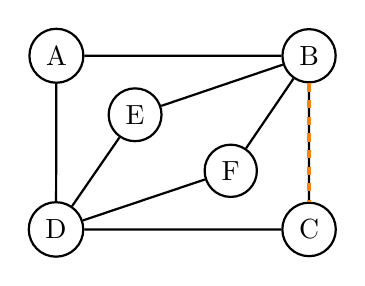
\begin{tikzpicture}[node distance={15mm}, thick] 
		\node[main] (A) {A}; 
		\node[main] (B) [right=2.5cm of A] {B};
		\node[main] (C) [below=1.5cm of B] {C}; 
		\node[main] (D) [left=2.5cm of C] {D};
		\node[main] (E) [below right=0.25cm and 0.5cm of A] {E}; 
		\node[main] (F) [above left=0.25cm and 0.5cm of C] {F}; 
		
		\begin{scope}[font=\tiny]
			\draw[main] (A) -- (B) -- (C) -- (D) -- (A);
			\draw[main] (D) -- (E) -- (B) -- (F) -- (D);
			
			\draw[BurntOrange, very thick, dashed] (B) -- (C);
		\end{scope}
	\end{tikzpicture} 
	
	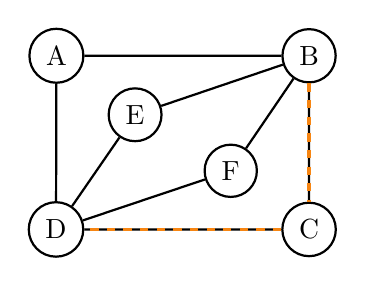
\begin{tikzpicture}[node distance={15mm}, thick] 
		\node[main] (A) {A}; 
		\node[main] (B) [right=2.5cm of A] {B};
		\node[main] (C) [below=1.5cm of B] {C}; 
		\node[main] (D) [left=2.5cm of C] {D};
		\node[main] (E) [below right=0.25cm and 0.5cm of A] {E}; 
		\node[main] (F) [above left=0.25cm and 0.5cm of C] {F}; 
		
		\begin{scope}[font=\tiny]
			\draw[main] (A) -- (B) -- (C) -- (D) -- (A);
			\draw[main] (D) -- (E) -- (B) -- (F) -- (D);
			
			\draw[BurntOrange, very thick, dashed] (B) -- (C) -- (D);
		\end{scope}
	\end{tikzpicture} 
	
	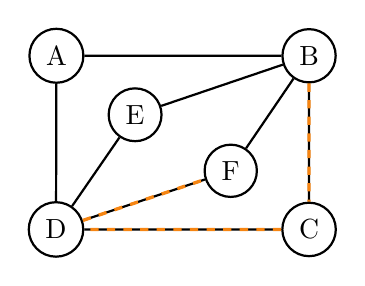
\begin{tikzpicture}[node distance={15mm}, thick] 
		\node[main] (A) {A}; 
		\node[main] (B) [right=2.5cm of A] {B};
		\node[main] (C) [below=1.5cm of B] {C}; 
		\node[main] (D) [left=2.5cm of C] {D};
		\node[main] (E) [below right=0.25cm and 0.5cm of A] {E}; 
		\node[main] (F) [above left=0.25cm and 0.5cm of C] {F}; 
		
		\begin{scope}[font=\tiny]
			\draw[main] (A) -- (B) -- (C) -- (D) -- (A);
			\draw[main] (D) -- (E) -- (B) -- (F) -- (D);
			
			\draw[BurntOrange, very thick, dashed] (B) -- (C) -- (D) -- (F);
		\end{scope}
	\end{tikzpicture} 
	
	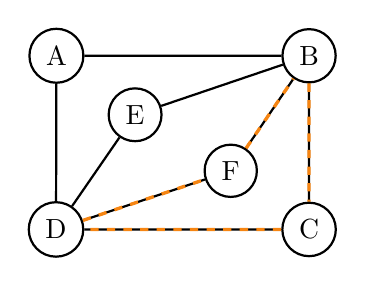
\begin{tikzpicture}[node distance={15mm}, thick] 
		\node[main] (A) {A}; 
		\node[main] (B) [right=2.5cm of A] {B};
		\node[main] (C) [below=1.5cm of B] {C}; 
		\node[main] (D) [left=2.5cm of C] {D};
		\node[main] (E) [below right=0.25cm and 0.5cm of A] {E}; 
		\node[main] (F) [above left=0.25cm and 0.5cm of C] {F}; 
		
		\begin{scope}[font=\tiny]
			\draw[main] (A) -- (B) -- (C) -- (D) -- (A);
			\draw[main] (D) -- (E) -- (B) -- (F) -- (D);
			
			\draw[BurntOrange, very thick, dashed] (B) -- (C) -- (D) -- (F) -- (B);
		\end{scope}
	\end{tikzpicture} 
	
	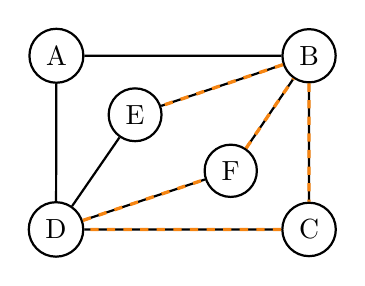
\begin{tikzpicture}[node distance={15mm}, thick] 
		\node[main] (A) {A}; 
		\node[main] (B) [right=2.5cm of A] {B};
		\node[main] (C) [below=1.5cm of B] {C}; 
		\node[main] (D) [left=2.5cm of C] {D};
		\node[main] (E) [below right=0.25cm and 0.5cm of A] {E}; 
		\node[main] (F) [above left=0.25cm and 0.5cm of C] {F}; 
		
		\begin{scope}[font=\tiny]
			\draw[main] (A) -- (B) -- (C) -- (D) -- (A);
			\draw[main] (D) -- (E) -- (B) -- (F) -- (D);
			
			\draw[BurntOrange, very thick, dashed] (B) -- (C) -- (D) -- (F) -- (B) -- (E);
		\end{scope}
	\end{tikzpicture} 
	
	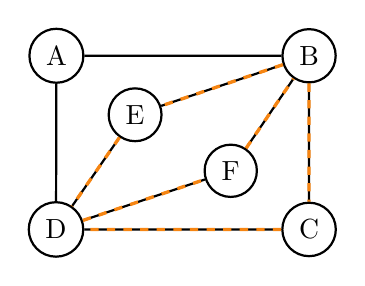
\begin{tikzpicture}[node distance={15mm}, thick] 
		\node[main] (A) {A}; 
		\node[main] (B) [right=2.5cm of A] {B};
		\node[main] (C) [below=1.5cm of B] {C}; 
		\node[main] (D) [left=2.5cm of C] {D};
		\node[main] (E) [below right=0.25cm and 0.5cm of A] {E}; 
		\node[main] (F) [above left=0.25cm and 0.5cm of C] {F}; 
		
		\begin{scope}[font=\tiny]
			\draw[main] (A) -- (B) -- (C) -- (D) -- (A);
			\draw[main] (D) -- (E) -- (B) -- (F) -- (D);
			
			\draw[BurntOrange, very thick, dashed] (B) -- (C) -- (D) -- (F) -- (B) -- (E) -- (D);
		\end{scope}
	\end{tikzpicture} 
	
	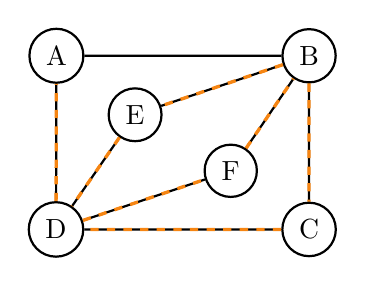
\begin{tikzpicture}[node distance={15mm}, thick] 
		\node[main] (A) {A}; 
		\node[main] (B) [right=2.5cm of A] {B};
		\node[main] (C) [below=1.5cm of B] {C}; 
		\node[main] (D) [left=2.5cm of C] {D};
		\node[main] (E) [below right=0.25cm and 0.5cm of A] {E}; 
		\node[main] (F) [above left=0.25cm and 0.5cm of C] {F}; 
		
		\begin{scope}[font=\tiny]
			\draw[main] (A) -- (B) -- (C) -- (D) -- (A);
			\draw[main] (D) -- (E) -- (B) -- (F) -- (D);
			
			\draw[BurntOrange, very thick, dashed] (B) -- (C) -- (D) -- (F) -- (B) -- (E) -- (D) -- (A);
		\end{scope}
	\end{tikzpicture}
	
	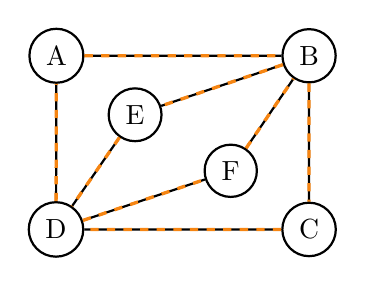
\begin{tikzpicture}[node distance={15mm}, thick] 
		\node[main] (A) {A}; 
		\node[main] (B) [right=2.5cm of A] {B};
		\node[main] (C) [below=1.5cm of B] {C}; 
		\node[main] (D) [left=2.5cm of C] {D};
		\node[main] (E) [below right=0.25cm and 0.5cm of A] {E}; 
		\node[main] (F) [above left=0.25cm and 0.5cm of C] {F}; 
		
		\begin{scope}[font=\tiny]
			\draw[main] (A) -- (B) -- (C) -- (D) -- (A);
			\draw[main] (D) -- (E) -- (B) -- (F) -- (D);
			
			\draw[BurntOrange, very thick, dashed] (B) -- (C) -- (D) -- (F) -- (B) -- (E) -- (D) -- (A) -- (B);
		\end{scope}
	\end{tikzpicture}
	
\end{document}